\PassOptionsToPackage{usenames,dvipsnames}{xcolor}% Periwinkle, ForestGreen...
\documentclass[class=article,border=2mm,tikz]{standalone}
\usepackage{amsmath}% \dfrac
\usetikzlibrary{calc}% to use ($(B)!(A)!(C)$)
% radius of the circumscribed circle in terms of the smaller circle r
% R = r (3+2*(n-1)*sqrt(3))/3

\tikzset{%
  declare function={R(\x)=(3+2*(\x-1)*sqrt(3))/3;},
  pics/circle pyramid/.style={code={%
      \tikzset{circle pyramid/.cd,#1}%
      \pgfkeysgetvalue{/tikz/circle pyramid/n}\n
      \pgfkeysgetvalue{/tikz/circle pyramid/r}\r
      % draw large circle of radius R
      \path[circle pyramid/bg] circle[radius={\r*R(\n)}];
      \foreach \x in {\n,...,1} {
        \draw[circle pyramid/fg]
          \ifnum\x=\n
            (-150:{\r*R(\n)-\r})
          \else
            (row)++(60:2*\r)
          \fi
          coordinate (row)%
            \ifnum\x>1
            foreach \y in {1,...,\the\numexpr\x-1} {
              % draw small circles of radius r
              circle[radius=\r]++(2*\r,0)
            }
            \fi
            circle[radius=\r];
        }
    }  
 },
  circle pyramid/.cd,
  n/.initial=2,
  r/.initial=1,
  bg/.style={draw,fill=black},
  fg/.style={draw,fill=white},
}

\tikzset{%
  mark point/.style={fill, draw, circle, minimum width=3pt, inner sep=0pt},
}

% case n = 4
\newcommand{\DataA}{
  \pgfmathsetmacro{\r}{1}% r=1
  \pgfmathsetmacro{\n}{4}% n=4
  \pgfmathsetmacro{\a}{2*\r*(\n-1)}% a
  \pgfmathsetmacro{\R}{(3+2*(\n-1)*sqrt(3))*\r/3}% R
  \pgfmathsetmacro{\x}{\R-\r}% 
  \pgfmathsetmacro{\y}{sqrt(3)/3*\r*(\n-1)}% 
  \pgfmathsetmacro{\Ax}{-(\n-1)*\r}% x-coord of A
  \pgfmathsetmacro{\Ay}{-\y}% y-coord of A
  \pgfmathsetmacro{\Bx}{+(\n-1)*\r}% x-coord of B
  \pgfmathsetmacro{\By}{-\y}% y-coord of B
  \pgfmathsetmacro{\Cx}{0}% x-coord of C
  \pgfmathsetmacro{\Cy}{\x}% y-coord of C
  \coordinate (O) at (0,0);
  \coordinate (A) at (\Ax,\Ay); 
  \coordinate (B) at (\Bx,\By);
  \coordinate (C) at (\Cx,\Cy);
}

% Case n = 2
\newcommand{\DataB}{
  \pgfmathsetmacro{\r}{1}% r=1
  \pgfmathsetmacro{\n}{2}% n=2
  \pgfmathsetmacro{\a}{2*\r*(\n-1)}% a
  \pgfmathsetmacro{\R}{(3+2*(\n-1)*sqrt(3))*\r/3}% R
  \pgfmathsetmacro{\x}{\R-\r}% 
  \pgfmathsetmacro{\y}{sqrt(3)/3*\r*(\n-1)}% 
  \pgfmathsetmacro{\Ax}{-(\n-1)*\r}% x-coord of A
  \pgfmathsetmacro{\Ay}{-\y}% y-coord of A
  \pgfmathsetmacro{\Bx}{+(\n-1)*\r}% x-coord of B
  \pgfmathsetmacro{\By}{-\y}% y-coord of B
  \pgfmathsetmacro{\Cx}{0}% x-coord of C
  \pgfmathsetmacro{\Cy}{\x}% y-coord of C
  \coordinate (O) at (0,0);
  \coordinate (A) at (\Ax,\Ay); 
  \coordinate (B) at (\Bx,\By);
  \coordinate (C) at (\Cx,\Cy);
}

\begin{document}

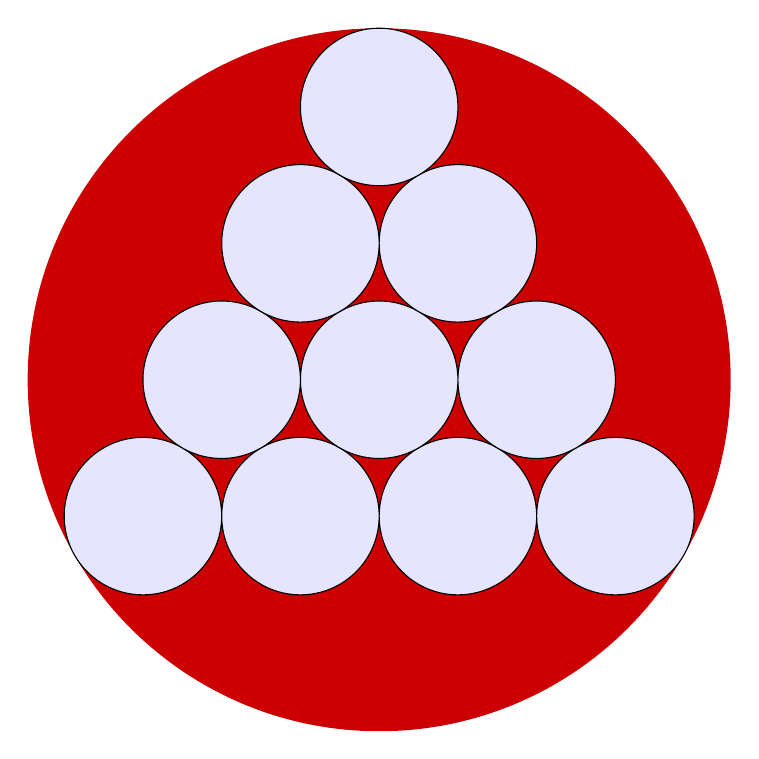
\begin{tikzpicture}[x=1cm,y=1cm]
  \path pic{circle pyramid={%
    n=4,
    bg/.style={fill=black!20!red},
    fg/.style={fill=blue!10!white}}}; 
\end{tikzpicture}


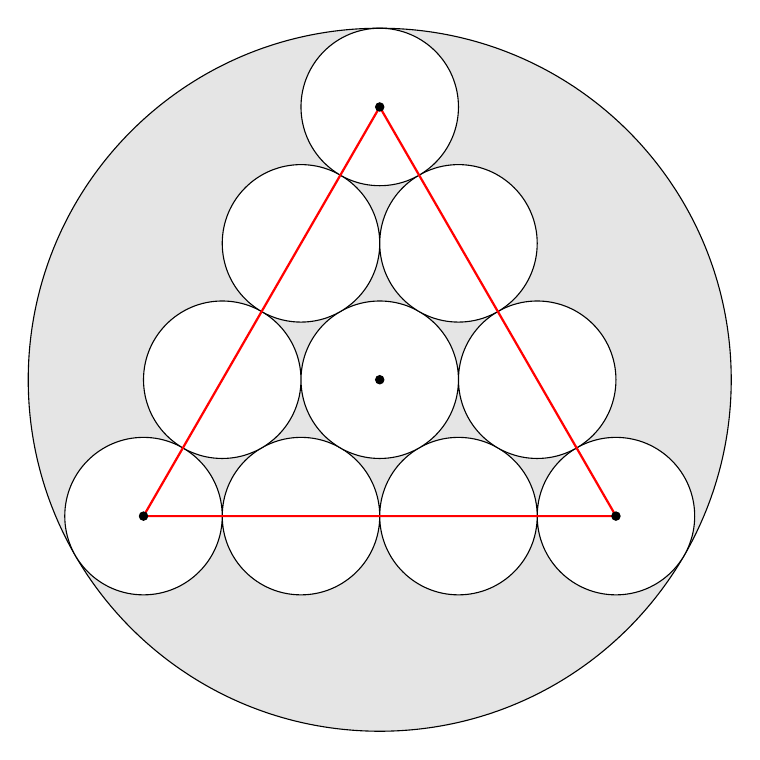
\begin{tikzpicture}[x=1cm,y=1cm]
  \DataA% makes coordinates available
  \path pic{circle pyramid={%
    n=4,
    bg/.style={fill=gray!20!white,draw=black}
  }}; 
  \draw [thick,red] (A) -- (B) -- (C) -- cycle;
  \foreach \point in {(O), (A), (B), (C)} {
    \node [mark point] at \point {};
  }
\end{tikzpicture}


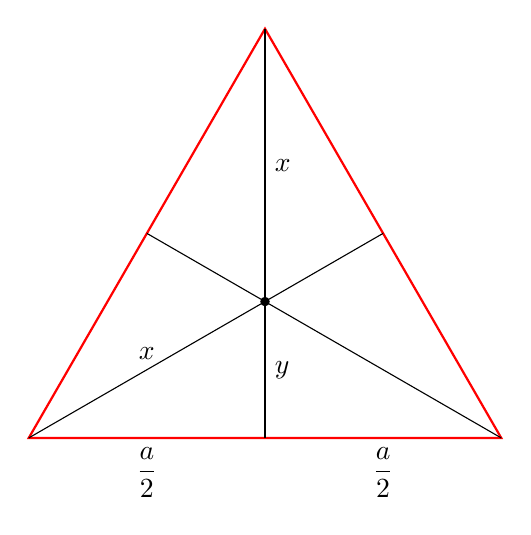
\begin{tikzpicture}[x=1cm,y=1cm]
  \DataA% makes coordinates available
  \node [mark point] at (O) {};
  \draw [thick,red] (A) -- (B) -- (C) -- cycle;
  \path (O) -- (A) node [midway,above] {$x$};
  \path (O) -- (C) node [midway,right] {$x$};
  \path (O) -- ($(A)!(C)!(B)$) node [midway,right] {$y$};
  \draw (C) -- ($(A)!(C)!(B)$);
  \draw (A) -- ($(B)!(A)!(C)$);
  \draw (B) -- ($(A)!(B)!(C)$);
  \path (A) -- ($(A)!(C)!(B)$) node [midway,below] {$\dfrac{a}{2}$};
  \path (B) -- ($(A)!(C)!(B)$) node [midway,below] {$\dfrac{a}{2}$};
\end{tikzpicture}


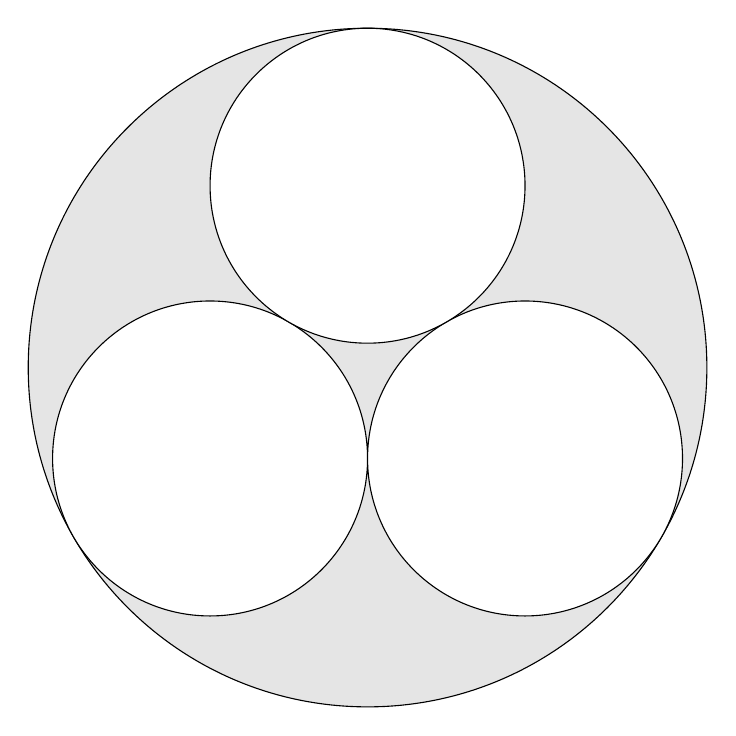
\begin{tikzpicture}[x=2cm,y=2cm]
  \path pic{circle pyramid={%
    n=2,
    bg/.style={fill=gray!20!white,draw=black}}};
\end{tikzpicture}


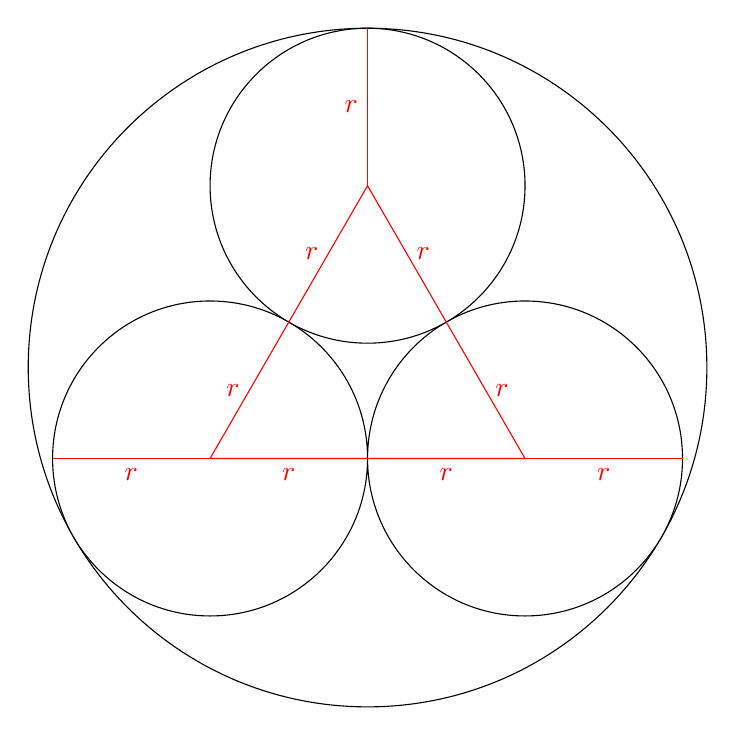
\begin{tikzpicture}[x=2cm,y=2cm]
  \DataB% makes coordinates available
  \path pic{circle pyramid={%
    n=2,
    bg/.style={draw=black}}}; 
  \draw [red] (A) -- (B) node [pos=0.25,below] {$r$} node [pos=0.75,below] {$r$} -- (C) node [pos=0.25,right] {$r$} node [pos=0.75,right] {$r$} -- (A) node [pos=0.25,left] {$r$} node [pos=0.75,left] {$r$};
  \draw [red] (A) --++ (-\r,0) node [pos=0.5,below] {$r$};
  \draw [red] (B) --++ (+\r,0) node [pos=0.5,below] {$r$};
  \draw [red] (C) --++ (0,+\r) node [pos=0.5,left] {$r$};
\end{tikzpicture}


\begin{tikzpicture}[x=1cm,y=1cm]
\foreach \z [count=\xi from 0] in {1, 0.646, 0.548, 0.502, 0.475, 0.458, 0.445, 0.436, 0.429, 0.424}{
  \pgfmathsetmacro{\y}{-floor(\xi/5)}
  \pgfmathsetmacro{\k}{mod(-\y,2)}
  \pgfmathsetmacro{\x}{4*\k-(2*\k-1)*mod(\xi,5)}
  \node [anchor=center] at (3*\x,3*\y) {
    \begin{tikzpicture}
      \node at (0,-1.3cm) {$n=\pgfmathparse{\xi+1}\pgfmathprintnumber{\pgfmathresult}$};
      \draw [fill=black,draw=black] (0,0) -- (90:1) arc(90:90-360*\z:1) -- cycle;
      \draw [black] (0,0) circle (1); 
    \end{tikzpicture}% 
    };
  }
\end{tikzpicture}


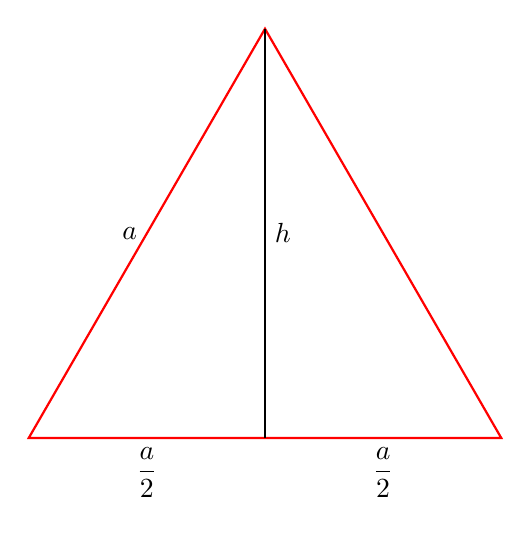
\begin{tikzpicture}[x=1cm,y=1cm]
  \DataA% makes coordinates available
  \draw [thick,red] (A) -- (B) -- (C) -- cycle;
  \draw (C) -- ($(A)!(C)!(B)$);
  \path (C) -- ($(A)!(C)!(B)$) node [midway,right] {$h$};
  \path (A) -- ($(A)!(C)!(B)$) node [midway,below] {$\dfrac{a}{2}$};
  \path (B) -- ($(A)!(C)!(B)$) node [midway,below] {$\dfrac{a}{2}$};
  \path (A) -- (C) node [midway,left] {$a$};
%  \path (B) -- (C) node [midway,right] {$a$};
\end{tikzpicture}

\end{document}
